% vim:encoding=utf8 ft=tex sts=2 sw=2 et:

\documentclass{classrep}
\usepackage[utf8]{inputenc}
\usepackage{color}
\usepackage{mathtools}

\studycycle{Informatyka, studia niestacjonarne, mgr II st.}
\coursesemester{I}

\coursename{Przetwarzanie obrazu i dźwięku}
\courseyear{2015/2016}

\courseteacher{mgr inż. Piotr Ożdżyński}
\coursegroup{Sobota, 14:15}

\author{
  \studentinfo{Jakub Antosik}{XXXXXX} \and
  \studentinfo{Andrzej Lisowski}{206087} 
}

\title{Zadanie 1: Szkielet aplikacji do przetwarzania i analizy obrazów, operacje podstawowe, usuwanie szumu,
modyfikacje histogramu, filtracja liniowa i nieliniowa, splot.}

\begin{document}
\maketitle

\section{Cel}
Celem zadania było zapoznanie się z metodami analizy i przetwarzania obrazów. W części implementacyjnej należało stworzyć program w wybranym przez siebie języku programowania, który będzie w stanie przeprowadzić różne operacje na obrazie. Pełen spis funkcjonalności zostanie przedstawiony w sekcji \textit{Wprowadzenie}.

\section{Wprowadzenie}
Obraz w pamięci komputera jest reprezentowany przez macierz pikseli. Sam piksel jest zaś najmniejszym elementem obrazu, mogącym przyjmować różne wartości liczb naturalnych:\\
\begin{itemize}
\item 0 - 7 dla obrazów 1-bitowych\\
\item 0 - 255 dla obrazów 8-bitowych (odcienie szarości)\\
\item 0 - 16777215 dla obrazów 24-bitowych (po 8 bitów na każdy kolor RGB)\\
\end{itemize}
Poniżej przedstawione zostały teoretyczne podstawy trasformacji, którym poddane zostały testowe dane.

\subsection{Podstawowe operacje przetwarzania obrazu}
Sekcja ta opisuje podstawowe operacje przetwarzania obrazów, często wykorzystywane w codziennym życiu.

\subsubsection{Zmiana jasności}
Zmiana jasności obrazu polega na dodaniu do wartości każdego piksela pewnej stałej liczby k. Jeżeli stała jest dodatnia, mówimy o zwiększaniu jasności, jeżeli jest ujemna - jasność jest zmniejszana. W momencie, w którym wynik przekroczy wartości brzegowe piksela, przypisuje się mu p$_{\text{min}}$ lub p$_{\text{max}}$ zgodnie z poniższym wzorem:
\[ p(i) =
  \begin{cases}
    p_{min} & \quad \text{jeżeli } i + k < 0\\
    i + k  & \quad \text{jeżeli } p_{min} \leq i+k \leq p_{max}\\
    p_{max}  & \quad \text{jeżeli } i + k > 0\\
  \end{cases}
\]
gdzie:\\
\textit{p(i)} - wartość piksela po zmianie jasności,\\
\textit{i} - wartość piksela przed zmianą jasności,\\
\textit{p$_{\text{min}}$} - minimalna wartość piksela, p$_{\text{min}}$ = 0,\\
\textit{p$_{\text{max}}$} - maksymalna wartość piksela,\\
\textit{k} - zmiana jasności.\\

\subsubsection{Zmiana kontrastu}
Zmiana kontrastu obrazu polega na zwiększeniu jasności jasnych pikseli przy jednoczesnym zmniejszeniu jasności ciemnych pikseli. Ciemne piksele należą do przedziału $\langle$0,$ \frac{p_{max}}{2}$), zaś jasne do przedziału $\langle$$ \frac{p_{max}}{2}$,$p_{max}$$\rangle$.\\
\\
Wzór wygląda następująco:
\[ p(i) =
  \begin{cases}
    i \div k  & \quad \text{jeżeli } 0 \leq i < \frac{p_{max}}{2}\\
    i \ast k  & \quad \text{jeżeli } \frac{p_{max}}{2} \leq i \leq p_{max}\\
    p_{max}  & \quad \text{jeżeli } i \ast k > p_{max}\\
  \end{cases}
\]
gdzie:\\
\textit{p(i)} - wartość piksela po zmianie kontrastu,\\
\textit{i} - wartość piksela przed zmianą kontrastu,\\
\textit{p$_{\text{max}}$} - maksymalna wartość piksela,\\
\textit{k} - współczynnik zmiany kontrastu.\\

\subsubsection{Wyznaczenie negatywu}
Negatyw jest przedstawieniem pikseli obrazu jako różnicy wartości maksymalnej i obecnej:\\
\\
\[p(i) = p_{max} - i\]
gdzie:\\
\textit{p(i)} - wartość piksela po wyznaczeniu negatywu,\\
\textit{i} - wartość piksela przed zmianą kontrastu,\\
\textit{p$_{\text{max}}$} - maksymalna wartość piksela.\\

\subsection{Podstawowe filtry}
Poniższa sekcja opisuje 2 podstawowe filtry, które podległy analizie - filtr ze średnią arytmetyczną oraz filtr medianowy.

\subsubsection{Filtr ze średnią arytmetyczną}
Filtr ze średnią arytmetyczną jest wykorzystywany w operacjach odszumiania obrazu. Algorytm polega na przypisaniu do nowej wartości pikseli średniej arytmetycznej badanego elementu oraz jego sąsiedztwa s. Sąsiedztwo może przyjmować wartości potęg kolejnych liczb nieparzystych większych od 1:\\
\[ s \in \{9,25,49,...\} \]
\[ p(i) = \frac{\displaystyle\sum_{x=-n}^{n}\displaystyle\sum_{y=-n}^{n} i_{x,y}}{s} \]
gdzie:\\
\textit{p(i)} - wartość piksela po nałożeniu filtru,\\
\textit{i} - wartość piksela przed nałożeniem filtru,\\
\textit{s} - maska filtru,\\
\textit{n} - rozpiętość maski filtru, obliczana ze wzoru:\\
\[ n = \frac{\sqrt{s}-1}{2} \]
\textit{x} - współrzędna x piksela na obrazie,\\
\textit{y} - współrzędna y piksela na obrazie.\\
\\
Należy pamiętać, że piksele poddawane filtracji nie mogą być elementami brzegowymi obrazu, więc:
\[ i_x + n \leq x_{max} \wedge i_x - n \geq x_{min} \wedge i_y + n \leq y_{max} \wedge i_y - n \geq y_{min} \]
gdzie:\\
\textit{i} - wartość piksela przed zmianą kontrastu,\\
\textit{x} - współrzędna x piksela na obrazie,\\
\textit{y} - współrzędna y piksela na obrazie,\\
\textit{x$_{\text{max}}$} - maksymalna wartość współrzędnej x na obrazie,\\
\textit{x$_{\text{min}}$} - minimalna wartość współrzędnej x na obrazie, x$_{\text{min}}$ = 0,\\
\textit{y$_{\text{max}}$} - maksymalna wartość współrzędnej y na obrazie,\\
\textit{y$_{\text{min}}$} - minimalna wartość współrzędnej y na obrazie, y$_{\text{min}}$ = 0.\\

\subsubsection{Filtr medianowy}
Filtr medianowy jest bardzo podobny do filtru ze średnią arytmetyczną. W tym przypadku jednak, nowa wartość piksela jest medianą badanego elementu praz jego sąsiedztwa s. Sąsiedztwo może przyjmować wartości potęg kolejnych liczb nieparzystych większych od 1:\\
\[ s \in \{9,25,49,...\} \]
\[ p(i) = M_{s} \]
gdzie:\\
\textit{p(i)} - wartość piksela po nałożeniu filtru,\\
\textit{M} - mediana,\\
\textit{s} - maska filtru.\\
\\
Należy pamiętać, że piksele poddawane filtracji nie mogą być elementami brzegowymi obrazu, więc:
\[ i_x + n \leq x_{max} \wedge i_x - n \geq x_{min} \wedge i_y + n \leq y_{max} \wedge i_y - n \geq y_{min} \]
gdzie:\\
\textit{i} - wartość piksela przed zmianą kontrastu,\\
\textit{n} - rozpiętość maski filtru, obliczana ze wzoru:\\
\[ n = \frac{\sqrt{s}-1}{2} \]
\textit{x} - współrzędna x piksela na obrazie,\\
\textit{y} - współrzędna y piksela na obrazie,\\
\textit{x$_{\text{max}}$} - maksymalna wartość współrzędnej x na obrazie,\\
\textit{x$_{\text{min}}$} - minimalna wartość współrzędnej x na obrazie, x$_{\text{min}}$ = 0,\\
\textit{y$_{\text{max}}$} - maksymalna wartość współrzędnej y na obrazie,\\
\textit{y$_{\text{min}}$} - minimalna wartość współrzędnej y na obrazie, y$_{\text{min}}$ = 0.\\

\subsection{Modyfikacje obrazu w oparciu o histogram}
Histogram umożliwia przedstawienie rozkładu pikseli o określonych wartościach na wykresie. Poniższa sekcja prezentuje modyfikacje obrazu na podstawie jego histogramu.

\subsubsection{Jednostajna wyjściowa gęstość prawdopodobieństwa}
Obliczana jest ze wzoru:
\[ g(f) = g_{min} + (g_{max} - g_{min}) \frac{1}{N} \displaystyle\sum_{m=0}^{f} H(m) \]
gdzie:\\
\textit{f} - wartość rozważanego kanału przed modyfikacją,\\
\textit{g} - wartość rozważanego kanału po modyfikacji,\\
\textit{g$_{\text{min}}$} - pożądana minimalna wartość przetwarzanego kanału,\\
\textit{g$_{\text{max}}$} - pożądana maksymalna wartość przetwarzanego kanału,\\
\textit{N} - suma pikseli na obrazie,\\
\textit{H(m)} - wartość histogramu dla wartości m kanału.\\

\subsubsection{Wyjściowa gęstość prawdopodobieństwa o postaci wykładniczej}
Obliczana jest ze wzoru:
\[ g(f) = g_{min} - \frac{1}{\alpha} ln (1 - \frac{1}{N} \displaystyle\sum_{m=0}^{f} H(m) \]
gdzie:\\
\textit{f} - wartość rozważanego kanału przed modyfikacją,\\
\textit{g} - wartość rozważanego kanału po modyfikacji,\\
\textit{g$_{\text{min}}$} - pożądana minimalna wartość przetwarzanego kanału,\\
\textit{$\alpha$} - współczynnik obiczany ze wzoru: TODO,\\
\textit{N} - suma pikseli na obrazie,\\
\textit{H(m)} - wartość histogramu dla wartości m kanału.\\

\subsubsection{Wyjściowa gęstość prawdopodobieństwa podana wzorem Raleigha}
Obliczana jest ze wzoru:
\[ g(f) = g_{min} + (2 \alpha^2 ln (\frac{1}{N} \displaystyle\sum_{m=0}^{f} H(m))^{-1})^\frac{1}{2} \]
gdzie:\\
\textit{f} - wartość rozważanego kanału przed modyfikacją,\\
\textit{g} - wartość rozważanego kanału po modyfikacji,\\
\textit{g$_{\text{min}}$} - pożądana minimalna wartość przetwarzanego kanału,\\
\textit{$\alpha$} - współczynnik obiczany ze wzoru: TODO,\\
\textit{N} - suma pikseli na obrazie,\\
\textit{H(m)} - wartość histogramu dla wartości m kanału.\\

\subsubsection{Wyjściowa gęstość prawdopodobieństwa określona przez potęgę 2/3}
Obliczana jest ze wzoru:
\[ g(f) = (g_{min}^\frac{1}{3} + (g_{max}^\frac{1}{3} - g_{min}^\frac{1}{3}) \frac{1}{N} \displaystyle\sum_{m=0}^{f} H(m))^3 \]
gdzie:\\
\textit{f} - wartość rozważanego kanału przed modyfikacją,\\
\textit{g} - wartość rozważanego kanału po modyfikacji,\\
\textit{g$_{\text{min}}$} - pożądana minimalna wartość przetwarzanego kanału,\\
\textit{g$_{\text{max}}$} - pożądana maksymalna wartość przetwarzanego kanału,\\
\textit{N} - suma pikseli na obrazie,\\
\textit{H(m)} - wartość histogramu dla wartości m kanału.\\

\subsubsection{Wyjściowa gęstość prawdopodobienstwa o postaci hiperbolicznej}
Obliczana jest ze wzoru:
\[ g(f) = g_{min}(\frac{g_{max}}{g_{min}})^{\frac{1}{N} \displaystyle\sum_{m=0}^{f} H(m)} \]
gdzie:\\
\textit{f} - wartość rozważanego kanału przed modyfikacją,\\
\textit{g} - wartość rozważanego kanału po modyfikacji,\\
\textit{g$_{\text{min}}$} - pożądana minimalna wartość przetwarzanego kanału,\\
\textit{g$_{\text{max}}$} - pożądana maksymalna wartość przetwarzanego kanału,\\
\textit{N} - suma pikseli na obrazie,\\
\textit{H(m)} - wartość histogramu dla wartości m kanału.\\

\subsection{Filtracja liniowa oparta o splot}
Poniższa sekcja przedstawia zbadane przekształcenia filtracji liniowej. Polega ona na modyfikacji pikseli obrazu poprzez nałożenie na nie maski filtrującej. Wzór przedstawia się następująco: 
\[ g(p,q) = \displaystyle\sum_{i=-M}^{M}\displaystyle\sum_{j=-M}^{M} h(i,j)x(p+i,q+j), p = M,2,...,P-M-1, q = M,2,...,Q-M-1 \]
gdzie:\\
\textit{x(p,q)} - wartość rozważanego kanału przed modyfikacją,\\
\textit{g(p,q)} - wartość rozważanego kanału po modyfikacji,\\
\textit{h(i,j)} - wartość maski filtru.\\

\subsubsection{Filtr dolnoprzepustowy}
Filtry dolnoprzepustowe są wykorzystywane do usuwania elementów o wysokiej częstotliwości. Dążą one to uśrednienia wartości sąsiadujących pikselów.
Wykorzystane maski:
\[
\frac{1}{9}
 \begin{pmatrix}
  1 & 1 & 1 \\
  1 & 1 & 1 \\
  1 & 1 & 1 \\
 \end{pmatrix}
\quad
\frac{1}{10}
 \begin{pmatrix}
  1 & 1 & 1 \\
  1 & 2 & 1 \\
  1 & 1 & 1 \\
 \end{pmatrix}
\quad
\frac{1}{16}
 \begin{pmatrix}
  1 & 2 & 1 \\
  2 & 4 & 2 \\
  1 & 2 & 1 \\
 \end{pmatrix}
\]

\subsubsection{Wyostrzanie krawędzi}
Poniższe maski zostały użyte do wyostrzenia krawędzi:
\[
 \begin{pmatrix}
  0 & -1 & 0 \\
  -1 & 5 & -1 \\
  0 & -1 & 0 \\
 \end{pmatrix}
\quad
 \begin{pmatrix}
  -1 & -1 & -1 \\
  -1 & 9 & -1 \\
  -1 & -1 & -1 \\
 \end{pmatrix}
\quad
 \begin{pmatrix}
  1 & -2 & 1 \\
  -2 & 5 & -2 \\
  1 & -2 & 1 \\
 \end{pmatrix}
\]

\subsubsection{Wydobywanie szczegółów z tła: N, NE, E, SE}
Wydobycie szczegółów z tła w kierunkach: północnym, północno-wschodnim, wschodnim i południowo-wschodnim zostało przebadane następującymi maskami:
\[
 \begin{pmatrix}
  1 & 1 & 1 \\
  1 & -2 & 1 \\
  -1 & -1 & -1 \\
 \end{pmatrix}
\quad
 \begin{pmatrix}
  1 & 1 & 1 \\
  -1 & -2 & 1 \\
  -1 & -1 & 1 \\
 \end{pmatrix}
\quad
 \begin{pmatrix}
  -1 & 1 & 1 \\
  -1 & -2 & 1 \\
  -1 & 1 & 1 \\
 \end{pmatrix}
\quad
 \begin{pmatrix}
  -1 & -1 & 1 \\
  -1 & -2 & 1 \\
  1 & 1 & 1 \\
 \end{pmatrix}
\]

\subsubsection{Wydobywanie szczegółów z tła: S, SW, W, NW}
Do wydobycia szczegółów z tła w kierunkach: południowym, południowo-zachodnim, zachodnim i północno-zachodnim zostało wykorzystane następujące maski:
\[
 \begin{pmatrix}
  -1 & -1 & -1 \\
  1 & -2 & 1 \\
  1 & 1 & 1 \\
 \end{pmatrix}
\quad
 \begin{pmatrix}
  1 & -1 & -1 \\
  1 & -2 & -1 \\
  1 & 1 & 1 \\
 \end{pmatrix}
\quad
 \begin{pmatrix}
  1 & 1 & -1 \\
  1 & -2 & -1 \\
  1 & 1 & -1 \\
 \end{pmatrix}
\quad
 \begin{pmatrix}
  1 & 1 & 1 \\
  1 & -2 & -1 \\
  1 & -1 & -1 \\
 \end{pmatrix}
\]

\subsubsection{Wydobywanie szczegółów z tła bez zdefiniowanego kierunku (laplasjan)}
Wydobycie szczegółów z tła bez zdefiniowanego kierunku jest możliwe przy nałożeniu następujących masek:
\[
 \begin{pmatrix}
  0 & -1 & 0 \\
  -1 & 4 & -1 \\
  0 & -1 & 0 \\
 \end{pmatrix}
\quad
 \begin{pmatrix}
  -1 & -1 & -1 \\
  -1 & 8 & -1 \\
  -1 & -1 & -1 \\
 \end{pmatrix}
\quad
 \begin{pmatrix}
  1 & -2 & 1 \\
  -2 & 4 & -2 \\
  1 & -2 & 1 \\
 \end{pmatrix}
\]

\subsubsection{Identyfikowanie linii}
Identyfikowanie linii na obrazie zostało zrealizowane po nałożeniu masek:
\[
 \begin{pmatrix}
  -1 & 2 & -1 \\
  -1 & 2 & -1 \\
  -1 & 2 & -1 \\
 \end{pmatrix}
\quad
 \begin{pmatrix}
  -1 & -1 & -1 \\
  2 & 2 & 2 \\
 -1 & -1 & -1 \\
 \end{pmatrix}
\quad
 \begin{pmatrix}
  -1 & -1 & 2 \\
  -1 & 2 & -1 \\
  2 & -1 & -1 \\
 \end{pmatrix}
\quad
 \begin{pmatrix}
  2 & -1 & -1 \\
  -1 & 2 & -1 \\
  -1 & -1 & 2 \\
 \end{pmatrix}
\]

\subsection{Filtracja nieliniowa}
//TODO

\subsubsection{Operator Robertsa (Wariant I)}
//TODO

\subsubsection{Operator Robertsa (Wariant II)}
//TODO

\subsubsection{Operator Sobela}
//TODO

\subsubsection{Operator Kirsha}
//TODO

\subsubsection{Operator Rosenfelda}
//TODO

\subsubsection{Operator Uolisa}
//TODO

\section{Opis implementacji}
Aplikacja została napisana w języku programowania Java. Wybór środowiska był podyktowany dużą ilością bibliotek mogących pomóc w realizacji zadania oraz osobistymi preferencjami członków zespołu. Warstwa GUI została realizowana przy użyciu standardowej bilbioteki graficznej Javy - Swing. Aplikacja wykorzystuje następujące bilbioteki zewnętrzne:
\begin{itemize}
\item \textit{JavaPlot.jar} - wykorzystywana do tworzenia histogramów; jest to javowa implementacja gnuplota 
\item \textit{log4j-1.2.17.jar} - wykorzystywana do obsługi logowania
\item \textit{slf4j-api-1.7.12.jar} - wykorzystywana do obsługi logowania
\item \textit{slf4j-log4j12-1.7.12.jar} - wykorzystywana do obsługi logowania
\end{itemize}

Poniżej przedstawiony został diagram UML klas znajdujących się w programie. Aby zachować czytelność, nie zamieszczono połączeń pomiędzy wywołaniami obiektów, a także ukryto informacje na temat metod i parametrów.

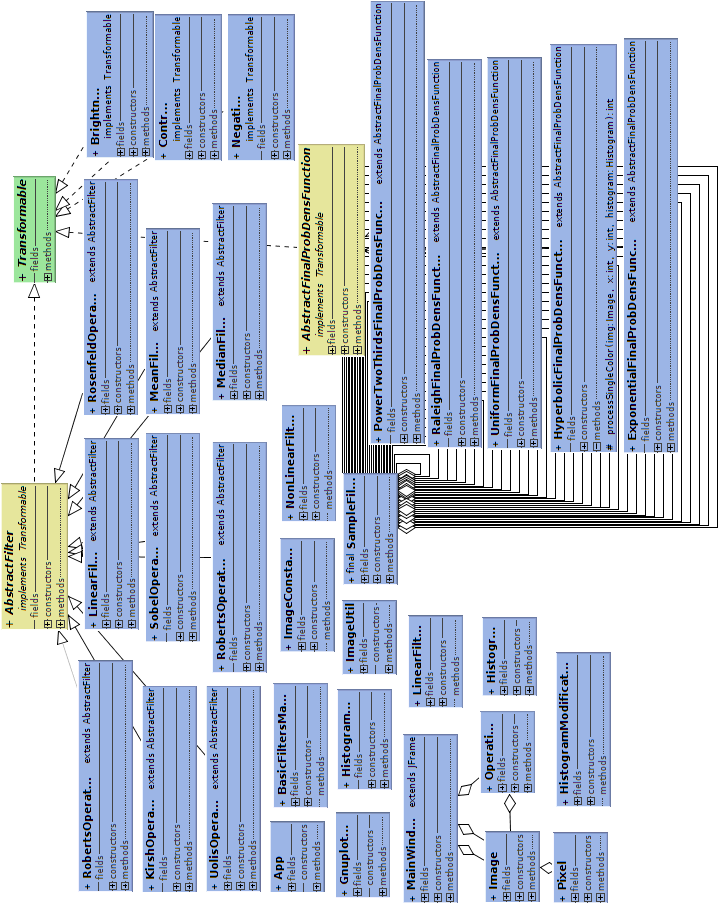
\includegraphics[scale=0.6]{uml_diagram.png}

\section{Materiały i metody}
{\color{blue}
W tym miejscu należy opisać, jak przeprowadzone zostały wszystkie badania,
których wyniki i dyskusja zamieszczane są w dalszych sekcjach. Opis ten
powinien być na tyle dokładny, aby osoba czytająca go potrafiła wszystkie
przeprowadzone badania samodzielnie powtórzyć w celu zweryfikowania ich
poprawności (a zatem m.in. należy zamieścić tu opis architektury sieci,
wartości współczynników użytych w kolejnych eksperymentach, sposób
inicjalizacji wag, metodę uczenia itp. oraz informacje o danych, na których
prowadzone były badania). Przy opisie należy odwoływać się i stosować do
opisanych w sekcji drugiej wzorów i oznaczeń, a także w jasny sposób opisać
cel konkretnego testu. Najlepiej byłoby wyraźnie wyszczególnić (ponumerować)
poszczególne eksperymenty tak, aby łatwo było się do nich odwoływać dalej.}

\section{Wyniki}
Sekcja przedstawia efekty przeprowadzonych badań. Przeanalizowane zostały wybrane obrazy 1-, 8- i 24-bitowe.

{\color{blue}
W tej sekcji należy zaprezentować, dla każdego przeprowadzonego eksperymentu,
kompletny zestaw wyników w postaci tabel, wykresów itp. Powinny być one tak
ponazywane, aby było wiadomo, do czego się odnoszą. Wszystkie tabele i wykresy
należy oczywiście opisać (opisać co jest na osiach, w kolumnach itd.) stosując
się do przyjętych wcześniej oznaczeń. Nie należy tu komentować i interpretować
wyników, gdyż miejsce na to jest w kolejnej sekcji. Tu również dobrze jest
wprowadzić oznaczenia (tabel, wykresów) aby móc się do nich odwoływać
poniżej.}

\section{Dyskusja}
{\color{blue}
Sekcja ta powinna zawierać dokładną interpretację uzyskanych wyników
eksperymentów wraz ze szczegółowymi wnioskami z nich płynącymi. Najcenniejsze
są, rzecz jasna, wnioski o charakterze uniwersalnym, które mogą być istotne
przy innych, podobnych zadaniach. Należy również omówić i wyjaśnić wszystkie
napotakane problemy (jeśli takie były). Każdy wniosek powinien mieć poparcie
we wcześniej przeprowadzonych eksperymentach (odwołania do konkretnych
wyników). Jest to jedna z najważniejszych sekcji tego sprawozdania, gdyż
prezentuje poziom zrozumienia badanego problemu.}
\section{Wnioski}
{\color{blue}W tej, przedostatniej, sekcji należy zamieścić podsumowanie
najważniejszych wniosków z sekcji poprzedniej. Najlepiej jest je po prostu
wypunktować. Znów, tak jak poprzednio, najistotniejsze są wnioski o
charakterze uniwersalnym.}


\begin{thebibliography}{0}
\end{thebibliography}
http://ftims.edu.p.lodz.pl/pluginfile.php/18220/mod_resource/content/1/Zadanie1.pdf
http://ics.p.lodz.pl/~tomczyk/available/po_en/second.html
https://en.wikibooks.org/wiki/LaTeX/Mathematics
https://pl.wikipedia.org/wiki/Filtracja_obraz%C3%B3w
{\color{blue} 
Na końcu należy obowiązkowo podać cytowaną w sprawozdaniu
literaturę, z której grupa korzystała w trakcie prac nad zadaniem (przykład na
końcu szablonu)}
\end{document}
